\section{Présentation du sujet de stage}
\addetoc{section}{Presentation of the internship}
\subsection{Descriptif général du projet Mach}
\addetoc{subsection}{General description of the Mach project}
\paragraph{ITEA Mach~\cite{mach}}
est un projet européen regroupant une vingtaine de partenaires dont AS+, le
CEA-LIST, l'INRA, Silkan, Thales Communications and security... L'objectif de ce
projet est de faciliter la programmation sur machines hybrides combinant CPU et
accélérateurs tels que GPU et Xeon-Phi, en partant d'une approche de type DSL
(Domain Specific Language) embarqué si besoin dans un langage hôte (DSeL). Pour
valider les frameworks mis en place, le projet dispose d’un certain nombre de
cas utilisateurs représentatifs de différents domaines : traitement d’image, du
signal, mécanique des fluides, biostatistiques, etc.

\paragraph{}
Le rôle d'AS+ est de fournir les technologies permettant de construire des
chaînes de compilation modulaires construites autour du compilateur LLVM et un
modèle d’exécution de type tâche pour des architectures hétérogènes en
s’appuyant sur les DSL mis en place pour chaque domaine. La Société travaille
plus particulièrement avec l’INRA et le CEA-LIST en langage R dans le domaine
des biostatistiques. L’INRA apporte les applications et le CEA-LIST apporte le
frontend de traduction du langage R vers vers une représentation intermédiaire
dont on a besoin dans notre chaîne de compilation, comme le montre la
figure~\ref{toolchain_fr}.

\begin{figure}[h!]
   \begin{center}
      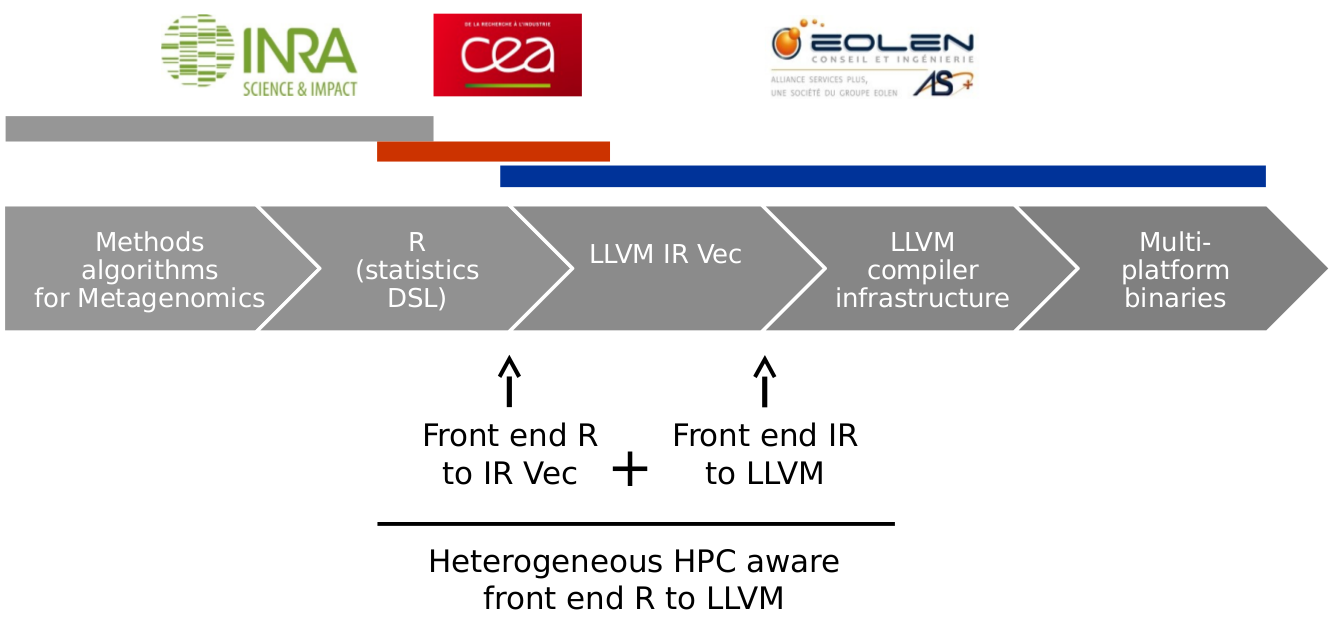
\includegraphics[width=135mm]{./images/toolchain_fr.png}
   \end{center}
   \caption{Chaîne d'outils du partenariat français~\cite{toolchain_fr}}
   \label{toolchain_fr}
\end{figure}

\paragraph{}
On peut décrire la chaîne de compilation développée par AS+ comme ceci : On
prend en entrée du code dans une version étendue du langage LLVM IR, annotée si
besoin pour faciliter la compilation. Le code passe par le tâchifieur
(Parallelizer) qui s'occupe de regrouper en tâches les instructions réalisées et
de les placer dans des procédures. Une fois le programme découpé en tâches, les
codes passent par les différents spécialisateurs pour être transformés en code
LLVM IR pur, avec les annotations adaptées à une architecture spécifique. Ils
peuvent ensuite passer dans la chaîne de compilation standard de LLVM pour être
optimisés et compilés sous forme binaire. La gestion de la mémoire et les appels
aux bibliothèques sont transformés en équivalents fournis par le runtime. Le
tout peut ensuite être regroupé dans un exécutable capable de tourner sur une
machine hétérogène.\\
La figure~\ref{backend_mach} résume tout cela.

\begin{figure}[h!]
   \begin{center}
      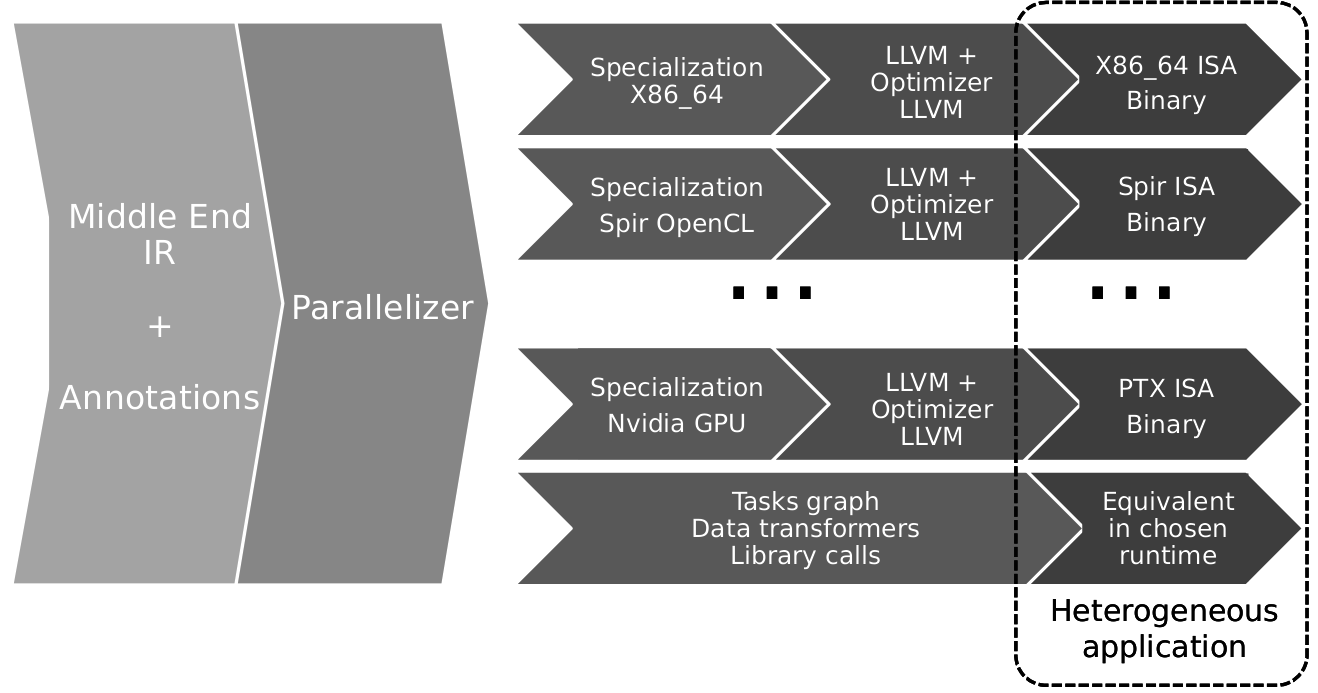
\includegraphics[width=135mm]{./images/backend_mach.png}
   \end{center}
   \caption{Back-end de l'outil de compilation \emph{Mach}~\cite{toolchain_fr}}
   \label{backend_mach}
\end{figure}

\subsection{Runtime}
\addetoc{subsection}{Runtime}
\subsubsection{Mach Runtime}
\addetoc{subsubsection}{Mach Runtime}
\paragraph{}
Nous avons donc besoin d'un runtime hétérogène, qui prendra en charge une
application conçue comme un ensemble de tâches, nous voulons donc lui laisser le
choix de gérer quand et dans quel ordre il va les exécuter, sachant qu'il
connait les accès mémoires de chaque tâche. Il pourra, par conséquent, se
construire un graphe de dépendance de données entre ces dernières, ainsi tout en
respectant un tant soit peu l'ordre dans lequel les tâches lui sont données, le
runtime pouvant les réordonner quand cela permet une exécution parallèle.\\
Le découpage en tâches de l’application permet une répartition de charge
dynamique sur les différentes ressources de calcul indépendamment de
l’application. Il doit donc être capable de déterminer les unités de calcul
disponibles. On lui incombe également la gestion de la mémoire et la gestion des
allocations et des copies mémoires dans le cas où des unités de calcul accèdent
à de la mémoire différente (comme le CPU et un GPU ou Xeon-Phi).

Il existe des runtimes qui répondent à nos attentes, nous allons donc en
utiliser un, StarPU. Mais nous allons tout de même définir une interface
d'abstraction pour limiter l'adhérence au runtime sous-jacent et nous permettre
d'ajouter des fonctionnalités absentes de ce dernier sans avoir à le modifier en
profondeur.

\subsubsection{STARPU}
\addetoc{subsubsection}{STARPU}
\paragraph{}
\sloppy
StarPU est un runtime par tâches pour systèmes multic\oe{}urs hétérogène
développé par l'équipe runtime de l'INRIA de Bordeaux~\cite{starpu}.

\fussy
Il peut gérer les systèmes multi-processeurs, GPU Nvidia en utilisant Cuda et
les différents périphériques répondant à OpenCL (GPU AMD ou Intel Xeon-Phi par
exemple).\\
Le runtime intègre également un gestionnaire de mémoire. Il est capable de gérer
les dépendances entre les tâches à l’aide des intentions fournies avec ces
tâches. Il fournit également la possibilité de découper les zones mémoires
enregistrées en sous parties, pour pouvoir, par exemple, permettre à des tâches
accédant à des zones différentes de la donnée de tourner en parallèle.

\subsection{LLVM}
\addetoc{subsection}{LLVM}
\subsubsection{Déscription}
\addetoc{subsubsection}{Description}
\paragraph{}
\sloppy
Anciennement appelé \og{} Low Level Virtual Machine \fg{} (Machine Virtuelle de
Bas Niveau en français), \emph{LLVM}~\cite{llvm} est un projet d'infrastructure
de compilation qui permet l'optimisation de code indépendamment de toute
plateforme et de tout langage à différentes étapes de la compilation ou à
l'exécution du programme avec un compilateur à la volée.\\
Le projet a débuté en 2000 en tant que projet de recherche sous la direction de
Vikram Adve et Chris Lattner à l'Université de l'Illinois à Urbana–Champaign. Il
est à présent distribué sous forme de logiciel libre avec une licence permissive
et il est écrit sous forme de bibliothèques réutilisables.

Il définit une séparation claire des phases de compilation, un langage
intermédiaire et un ensemble de back-end pouvant générer du code pour une
architecture spécifique.\\
Il propose aussi depuis sa version 2.6 le compilateur Clang pour les langages C,
C++, Objective-C et Objective-C++.\\
Ce front-end se charge de traduire le code en langage intermédiaire de plus bas
niveau, le c\oe{}ur de LLVM applique ensuite des passes de transformation et
d'optimisation de code, et le back-end, le code en assembleur pour une
architecture spécifique.

\paragraph{}
La modularité est un concept clés dans LLVM, grâce à cette architecture, l'ajout
de la prise en charge d'un nouveau langage de haut niveau est réduit à écrire le
front-end de traduction vers le LLVM IR et la prise en charge d'un nouveau
processeur avec le back-end correspondant. Mais LLVM impose cette séparation des
étapes de manière formelle : le seul outil de communication entre les étapes est
le langage LLVM IR.

\subsubsection{Pass}
\addetoc{subsubsection}{Pass}
\paragraph{}
La partie centrale fonctionne par l'application d’un ensemble de passes. Il y a
deux types de passes dans LLVM : les passes d’analyse, qui génèrent des
statistiques utilisables par d’autres passes sans modification du code ; et les
passes de transformations, qui modifient le code principalement pour l'optimiser
en se basant potentiellement sur les statistiques générées par le premier type
de passe. On peut indiquer des dépendances entre les passes. Celles-ci peuvent
nécessiter le résultat d’une autre passe ou bien invalider le travail d’une
autre, qui sera à exécuter à nouveau.

\subsubsection{IR}
\addetoc{subsubsection}{IR}
\paragraph{}
Le langage intermédiaire utilisé par LLVM est un langage d'assemblage sous forme
SSA (Static Single Assignment), c'est-à-dire qu'on ne peut affecter une valeur à
un registre qu'une seule fois. C'est un langage fortement typé qui possède un
nombre infini de registres.

Ce langage peut être utilisé sous trois formats de représentation : la
représentation mémoire, pour être utilisée par les outils de compilation ; le
format bitcode, pour être stocké sur disque ; et le format assembleur pour être
humainement lisible.

\subsection{IR Étendu}
\addetoc{subsection}{Extended IR}
\paragraph{}
En dépit de tout ce que nous offre le langage LLVM IR, il manque certaines
caractéristiques et manipulations que nous allons énoncer.

\subsubsection{ALV (Vecteur de taille arbitraire)}
\addetoc{subsubsection}{ALV (Arbitrary Lenght Vector)}
\paragraph{}
L'intérêt de ces vecteurs de tailles arbitraires est de simplifier la
compilation en laissant au module de spécialisation le soin de faire tenir
l'instruction dans l'unité vectorielle gérée par le matériel ciblé sans avoir à
préciser de taille au préalable, étant donné que la majorité des architectures
matérielles sont de type SIMD(Single Instruction Multiple Data)/SIMT(Single
Instruction Multiple Thread), une même instruction est donc appliquée sur un
vecteur de données en parallèle, ou à un sous-ensemble de vecteur avec
masquage.\\
Les ALV sont marqués de taille 0 en IR. Ils sont utiles pour gérer les données
spécifiques lors des instructions de chargement/stockage (load/store). Toutes
les opérations sur les vecteurs classiques sont supportées sur les ALV.

Il a fallut pour cela patcher LLVM afin de lui faire accepter les vecteurs de
taille nulle.

\subsubsection{ND array}
\addetoc{subsubsection}{ND array}
\paragraph{}
Ces tableaux à $n$ dimensions sont inspirés de la bibliothèque \emph{NumPy} de
\emph{Python}. Ces conteneurs sont transparents pour chaque types de données.
Ils offrent un concept de vue, c'est-à-dire que plusieurs ND array peuvent se
partager les mêmes données et y travailler et accéder de manières différentes.
Des fonctions de manipulation sont donc implémentées dans le runtime pour gérer
la copie, l'extraction, etc.\ de données de ces conteneurs.

\subsubsection{Marqueur d'Intents}
\addetoc{subsubsection}{Intents marker}
\paragraph{}
On les ajoute dans la déclaration d'une tâche, ils permettent de définir le type
d'accès sur un tableau : lecture seule, écriture seule, lecture/écriture ou
\emph{scratchpad}. Ce dernier est un cas particulier de vecteurs, on l'insère
comme premier argument dans toutes les tâches spécialisées, il nous permet de
stocker certaines données telles que la taille des dimensions des ND array, ou
le décalage à effectuer pour la vue. Il sert aussi de stockage temporaire des
résultats partiels lors d'une réduction parallèle.

\subsubsection{Fonctions particulières\label{particular_function}}
\addetoc{subsubsection}{Special Function}
\paragraph{}
On définit trois types de tâches en se basant sur une autre notion de la
bibliothèque \emph{NumPy}, les \emph{ufunc}, \emph{rfunc} et \emph{sfunc}. Cette
information est passée dans les métadonnées pour exprimer des concepts sur la
mise en \oe{}uvre des tâches.

\begin{itemize}
\item \emph{ufunc} (Universal function), est une fonction opérant sur des ND
array élément par élément.

\item \emph{rfunc} (Reduce function), est une opération de réduction
s'appliquant à tous les éléments d'un vecteur. Le ND array en entrée peut être
directement le résultat d'une fonction optionnelle \emph{ufunc}.

\item \emph{sfunc} (Scan function), est une opération de réduction cumulative
sur un vecteur.
\end{itemize}

\subsection{État d'avancement du projet Mach}
\addetoc{subsection}{Mach project progress}
\paragraph{}
Le projet \emph{Mach} n'en est pas à ses débuts, des passes de transformation de
code sont déjà implémentées. La première était la passe de spécialisation
\emph{Cuda}, où l'on retrouve les mêmes principes qu'en \emph{OpenCl}, c'est
d'ailleurs sur cette dernière que je base mon travail, les autre passes sont
définies ainsi :
\begin{description}
\item[PrototypeArgPacker] Créer une nouvelle fonction ayant la bonne signature.
\item[CallSiteTransform] Transformer l'appel de l’ancienne fonction à la nouvelle.
\item[IntentsAnalyser] Ajout des marqueurs d'intents sur les tableaux.
\item[TaskAnalysis] Analyse des tâches spécialisées.
\item[InitImplementWriter] Génération d'une fonction d'initialisation qui ajoute
   une référence de l'implémentation au runtime.
\item[MaskLowering] Appel aux intrinsèques de masquage scalaire.
\item[X86Specializer] Spécialisateur de code X86.
\end{description}

\subsection{KFE}
\addetoc{subsection}{KFE}
\paragraph{}
Les premiers codes permettant de tester le bon fonctionnement des passes de
spécialisateurs était écrit en langage LLVM, en raison de non disponibilité du
frontend R qui est encore sous développement, un autre frontend de compilation à
donc été implémenté temporairement prenant en entrée un code écrit en \og{} K
\fg{}, un langage inventé proche de la syntaxe \emph{C} qui nous permettrait
d'écrire un code de manière plus commode, et dont il était plus simple de lui
intégré les différents concept attendu dans la chaîne.
